\documentclass[lettersize,journal]{IEEEtran}
\usepackage{amsmath,amsfonts}
\usepackage{algorithmic}
\usepackage{algorithm}
\usepackage{array}
\usepackage[caption=false,font=normalsize,labelfont=sf,textfont=sf]{subfig}
\usepackage{textcomp}
\usepackage{stfloats}
\usepackage{url}
\usepackage{verbatim}
\usepackage{graphicx}
\usepackage{cite}
\usepackage{BookTabs}
\usepackage{siunitx}
\usepackage{gensymb}
\hyphenation{op-tical net-works semi-conduc-tor IEEE-Xplore}
% updated with editorial comments 8/9/2021

\begin{document}
	
	\title{Pycnometry and Continuous Distillation of Ethanol-Water mixtures}
	
	\author{Joseph Zimmerman}
	% <-this % stops a space
	
	
	
	\maketitle
	
	\begin{abstract}
		In this paper, two experiments were conducted on ethanol-water mixtures. A pycnometer and quartz-tubed densitometer were used to determine liquid densities across a variety of compositions of ethanol and water. Alcohol-gauging tables from the US Alcohol and Tobacco Tax and Trade Bureau (TTB) were used to correlate theoretical densities of various compositions of ethanol and water at various temperatures to apparent proofs at 60F and finally correct to true proof and mole fraction of ethanol. Densities, measured through the pycnometer and densitometer, were compared. 
	\end{abstract}
	
	\begin{IEEEkeywords}
		Article submission, IEEE, IEEEtran, journal, \LaTeX, paper, template, typesetting.
	\end{IEEEkeywords}
	
	\section{Introduction}
	\IEEEPARstart{P}{ycnometry} is a fundamental laboratory technique used to determine the density of solid or liquid substances by measuring their mass and volume and comparing them to a known volume. A pycnometer—a calibrated glass flask with a defined volume—is filled with the sample, and its mass is compared to the mass of the same flask filled with a reference fluid (water in our case). Digital densitometers can also be used to determine the density of a solution. Our digital densitometer measures density through a vibrating "U-Tube". The sample is introduced into a U-shaped borosilicate glass tube that is being excited to vibrate at its characteristic frequency electronically. The characteristic frequency changes depending on the density of the sample. Through determination of the characteristic frequency the density of the sample can be calculated. In the first part of our experiment, we determined the densities of various compositions of ethanol-water through pycnometry and a digital densitometer. Alcohol-gauging tables from the US Alcohol and Tobacco Tax and Trade Bureau (TTB) were used to correlate theoretical densities of various compositions ranging from pure ethanol to pure water at various temperatures to apparent proofs at 60F and finally correct to extract true proof and mole fraction of ethanol.
	\newline
	\newline
	\-\hspace{0.6cm}This theoretical array of densities and corresponding mole fractions were then used in the second part of the lab, where we performed a continuous distillation of an ethanol-water mixture at two different reflux ratios, 4 and 5 in our case. 
	
	\section{Theory}
	\subsection{Pycnometry}
	The pycnometer used in our experiment was a Kimble KiMax pycnometer. By measuring the mass of the empty pycnometer, the mass of the pycnometer filled with water (our reference fluid), the known density of water, and the mass of the pycnometer filled with the experimental solution, the density of the experimental solution can be determined by \cite{ref1}. 
	\begin{equation}
		\label{deqn_ex1}
		V = \frac{m_{w}-m_{e}}{\rho_{water}(t)} = \frac{m_{sample}-m_{e}}{\rho_{sample}}
	\end{equation}
	where $m_{w}$ is the mass of the pycnometer filled with water, $m_{e}$ is the mass of the empty pycnometer, $\rho_{water}(t)$ is the density of water at temperature T, and $\rho_{sample}$ is the density of the sample at T. This equation can be arranged to solve for $\rho_{sample}$.
	\begin{equation}
		\label{deqn_ex2}
		\rho_{sample}  = \frac{m_{sample} - m_{empty}}{m_{water}-m_{sample}}\cdot\rho_{water}(T)
	\end{equation}
	
	\subsection{Gauging alcohol with TTB tables}
	Table 6 from the TTB correlates specific gravities of ethanol-water mixtures at 60$\degree$ F to proofs. In order to obtain proofs at other temperatures, one must convert the measured density ($\rho_{1}$) at a given temperature (T1) to the hypothetical density ($\rho_{2}$) that a glass hydrometer would indicate if calibrated at the standard 60$\degree F$ reference temperature:
	
	\begin{equation}
		\label{deqn_ex3}
		\rho_{2} = \rho_{1} (1 + \alpha(T_{1} - 60\degree F))
	\end{equation}
	where $\alpha$ is the coefficient of thermal expansion for the hydrometer material (typically 25 $\cdot$ $\frac{10\textsuperscript{-6}}{\degree C}$ for glass).
	At this corrected density, specific gravity can be calculated using the reference density of water at 60, $\degree C$ 0.99904 g/cc. Then, Table 6 can be interpolated through a truncated Taylor series expansion to retrieve an apparent proof, $C_{2}$, implemented as equation 1 in python:
	 
	\begin{equation}
		\label{deqn_ex4}
		C_{2} = f(\gamma_{1},T1) = [f + (\gamma_{1}-\gamma_{R})\frac{\partial f}{\partial \gamma} ] 
	\end{equation}
	where $\gamma_{1}$ is the specific gravity of the sample corrected to 60$\degree F$
	This apparent proof still has instrument and sample temperature effects, so it must be corrected to a true proof using TTB Table 1. The computed apparent proof $C_{2}$ is rounded down to the nearest integer and used as a reference for interpolation of Table 1.
	\begin{equation}
		\label{deqn_ex5}
		C_3 = C_2 + (C_2 - C_R) \frac{\partial f}{\partial C}\bigg|_{C_R, T_R} + (T_1 - T_R) \frac{\partial C}{\partial T}\bigg|_{C_R, T_R}
	\end{equation}
	where $C_{3}$ is the estimated true proof of the mixture corrected for temperature, $T_{1}$. $C_{R}$ and $T_{R}$ are reference proofs and temperatures from values corresponding to the rounded-down $C_{2}$
	\begin{equation}
		\label{deqn_ex5.5}
		\kappa = \left(\omega^2 + \frac{k}{4}\right) \frac{m v}{P_0 A^2} \\
	\end{equation}
	Kappa can be determined experimentally.
	
	\subsection{Error Propagation}
	\subsubsection{Mass of weights added}
	The 6 different masses added to the piston to perform the calibration and oscillations were taken as the average mass across three measurements. Uncertainty of the masses were computed through a 95\% confidence interval, with N = 3.
	\subsubsection{Applied Pressures}
	Uncertainty in pressures were calculated according to the master equation for error propagation (lec 1.2). The diameter of the piston was given, so the only uncertainties that arose were propagated from uncertainties in mass measurements. 
	\begin{equation}
		\label{deqn_ex6}
		F = m \cdot g
	\end{equation}
	
	\begin{equation}
		\label{deqn_ex7}
		P = \frac{F}{A} \Rightarrow \frac{4m \cdot g}{\pi \cdot D^2}
	\end{equation}
	\begin{equation}
		\label{deqn_ex8}
		\delta P = \sqrt{{\frac{\partial P}{{\partial}^2 m}}^2 \cdot {\delta m}^2}  
	\end{equation}
	\subsubsection{Calibration Curve}
	The uncertainty in the slope of the calibration curve was determined through the following uncertainty propagation equations for a linear regression.
	\begin{equation}
		\label{eq:delta-n}
		\Delta \equiv N \left[\left(\sum_{i=1}^N P_i^2\right) - \left(\sum_{i=1}^N P_i\right)^2\right]
	\end{equation}
	\begin{equation}
		\label{eq:delta-y}
		\delta\frac{mV}{9V} = \sqrt{\frac{1}{N-2}\sum_{i=1}^N (\frac{mV}{9V}_i - b - mP_i)^2}
	\end{equation}
	\begin{equation}
		\label{eq:delta-m}
		\delta m = \delta \frac{mV}{9V} \sqrt{\frac{N}{\Delta}}
	\end{equation}
	where $\delta$m is the uncertainty in the calibration curve, in dimensions comparable to PendoTec's specification sheet for this case.
	\subsubsection{Kappa}
	\begin{equation}
		\label{deqn_ex10}
		\kappa = \left(\omega^2 + \frac{k}{4}\right) \frac{m v}{P_0 A^2} \\
	\end{equation}
	\begin{equation}
		\label{deqn_ex10}
		\delta\kappa = \sqrt{\left(\frac{d\kappa}{dm}\right)^2 (\delta m)^2 + \left(\frac{d\kappa}{dA}\right)^2 (\delta A)^2}
	\end{equation}
	
	
	\section{Experimental Methods}
	\subsection{Calibration}
	The pressure sensor was calibrated using air as a fluid by taking multiple voltage measurements of static pressure with 6 combinations of weights (with one of them being the unweighted plunger) added to the piston. Voltage readouts were recorded for each weight. Voltage was then plotted over pressure, then the pressure sensor calibration was calculated in units of [mV/psi/9V] and compared to the manufacturer's stated value.
	The data acquisition system (DAS) was configured and tested to ensure proper operation.
	\subsection{Ruchardt Experiment}
	The Ruchardt experiment was first conducted with air as the internal fluid across 4 different initial pressures. The piston height was set to 60mm every trial to ensure than the volume remained constant between trials, although our apparatus had considerable leakage. \\With the DAS running, oscillations were induced by pressing and abruptly releasing the piston.
	Oscillations containing 5 peaks or more were considered acceptable. Three acceptable trials were recorded for every weight value.
	
	The experiment was then repeated, using Argon and CO2 instead of air. Before conducting the experiment, the air in the apparatus was purged twice with the respective gas. Three trials were conducted for each of the four weights tested, accepting oscillations with five peaks or more.
	\section{Results}
	\subsection{Calibration}
	The calibration value was determined from the slope of the linear regression of recorded voltages, in mV, against varied pressures, in psi. This value was divided by 9V to match PendoTec specifications  to be 0.270756 $\pm$ 0.0000001 $\frac{mV}{psi\cdot9V}$. This value was used to determine the pressure in the apparatus from voltage readings in the following Ruchardt experiments
	
	\begin{figure}[!t]
		\centering
		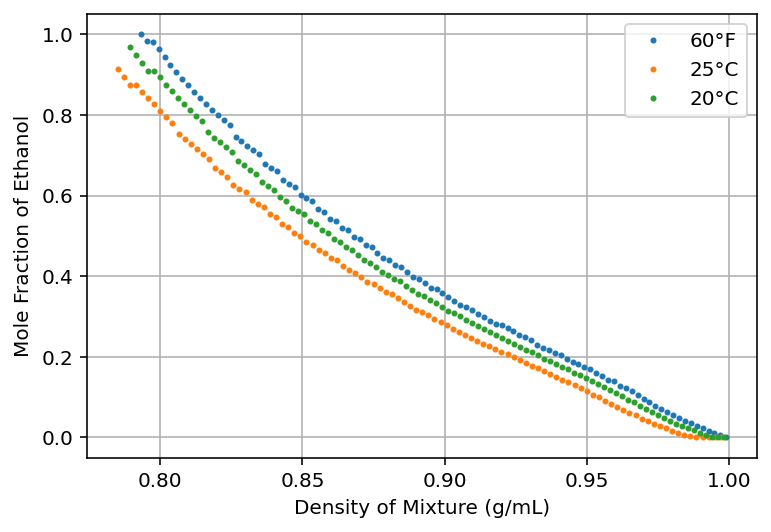
\includegraphics[width=3.6in]{fig1}
		\caption{Measured voltage readings from a PendoTec single-use pressure sensor recorded at various static pressures from a gas piston apparatus containing air. Static pressures were induced by adding weights of [84.248 $\pm$ 0.007g; 164.817 $\pm$ 0.007g; 239.434 $\pm$ 0.002g; 328.00 $\pm$ 0.01g and 402.531 $\pm$ 0.003g.] to the apparatus and appear in the figure from left to right. Error bars were calculated based on a 95\% confidence interval of recorded voltage readings in mV across three trials for each pressure (N=2). Uncertainty }
		\label{fig_1}
	\end{figure}
	\begin{table*}[!htbp]
		\centering
		\caption{Gas Properties}
		\label{tab:gas_properties}
		\begin{tabular}{lcccccc}
			\toprule
			Gas & Condition & $P_0$ (Pa) & $C$ (Pa) & $\kappa$ (s$^{-1}$) & $\omega$ (rad s$^{-1}$) & $\phi$ (rad) \\
			\midrule
			Air & Empty & $102171.80 \pm 7.20$ & $4518.24 \pm 886.00$ & $37.53 \pm 2.97$ & $217.85 \pm 2.87$ & $-9.62 \pm 3.02$ \\
			& 1 Weight & $103076.35 \pm 2.59$ & $2061.26 \pm 545.07$ & $14.59 \pm 1.03$ & $118.06 \pm 0.64$ & $-10.88 \pm 7.99$ \\
			& 2 Weight & $103389.06 \pm 1.81$ & $4264.83 \pm 513.42$ & $10.45 \pm 0.76$ & $90.98 \pm 0.63$ & $-8.53 \pm 6.94$ \\
			& 3 Weight & $104821.81 \pm 12.52$ & $-1212.16 \pm 513.84$ & $10.03 \pm 0.56$ & $79.06 \pm 0.73$ & $-15.93 \pm 9.20$ \\
			Argon & Empty & $102269.40 \pm 4.39$ & $-1487.97 \pm 3403.32$ & $16.59 \pm 4.37$ & $207.72 \pm 0.38$ & $-12.77 \pm 6.63$ \\
			& 1 Weight & $103093.24 \pm 3.53$ & $23.81 \pm 945.56$ & $15.69 \pm 0.08$ & $120.07 \pm 0.51$ & $-15.62 \pm 4.69$ \\
			& 2 Weight & $104000.11 \pm 21.84$ & $1201.48 \pm 2621.70$ & $17.28 \pm 1.22$ & $80.95 \pm 0.35$ & $-31.05 \pm 8.21$ \\
			& 3 Weight & $104882.66 \pm 36.64$ & $349.51 \pm 7984.72$ & $14.13 \pm 0.50$ & $77.39 \pm 0.91$ & $-15.90 \pm 11.16$ \\
			CO$_2$ & Empty & $102304.81 \pm 15.52$ & $882.70 \pm 1867.09$ & $32.71 \pm 5.98$ & $178.53 \pm 1.66$ & $-22.61 \pm 15.44$ \\
			& 1 Weight & $102216.12 \pm 3.98$ & $890.54 \pm 3907.62$ & $14.78 \pm 3.93$ & $106.12 \pm 2.15$ & $-22.41 \pm 23.91$ \\
			& 2 Weight & $103976.97 \pm 3.03$ & $-1087.62 \pm 2016.17$ & $9.09 \pm 1.17$ & $83.14 \pm 0.42$ & $-25.64 \pm 13.47$ \\
			& 3 Weight & $104000.26 \pm 14.20$ & $-6199.73 \pm 518.83$ & $6.59 \pm 1.27$ & $68.67 \pm 0.14$ & $-13.64 \pm 11.07$ \\
			\bottomrule
		\end{tabular}
	\end{table*}
	
	
	\begin{figure*}[!t]
		\centering
		\subfloat[]{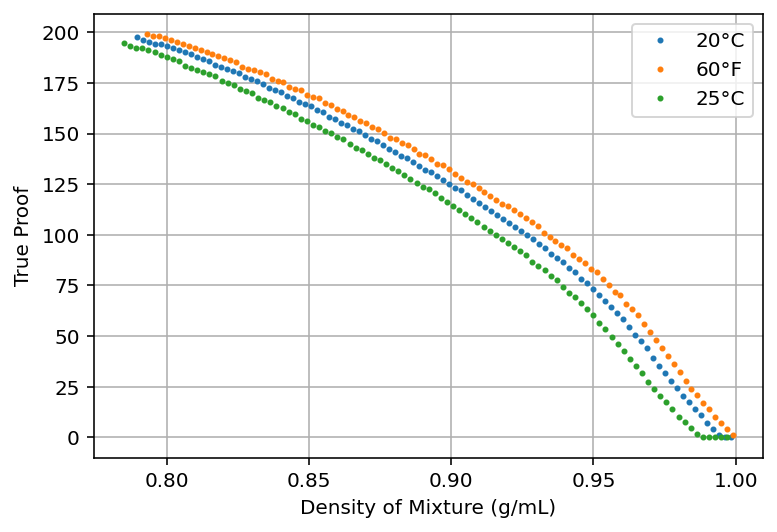
\includegraphics[width=5in]{fig2}%
			\label{a}}
		\hfil
		\caption{Dae. Ad quatur autat ut porepel itemoles dolor autem fuga. Bus quia con nessunti as remo di quatus non perum que nimus. (a) Case I. (b) Case II.}
		
	\end{figure*}
	
	Note that often IEEE papers with multi-part figures do not place the labels within the image itself (using the optional argument to $\backslash${\tt{subfloat}}[]), but instead will
	reference/describe all of them (a), (b), etc., within the main caption.
	Be aware that for subfig.sty to generate the (a), (b), etc., subfigure
	labels, the optional argument to $\backslash${\tt{subfloat}} must be present. If a
	subcaption is not desired, leave its contents blank,
	e.g.,$\backslash${\tt{subfloat}}[].
	
	
	
	
	\section{Discussion}
	Note that, for IEEE-style tables, the
	$\backslash${\tt{caption}} command should come BEFORE the table. Table captions use title case. Articles (a, an, the), coordinating conjunctions (and, but, for, or, nor), and most short prepositions are lowercase unless they are the first or last word. Table text will default to $\backslash${\tt{footnotesize}} as
	the IEEE normally uses this smaller font for tables.
	The $\backslash${\tt{label}} must come after $\backslash${\tt{caption}} as always.
	
	
	\begin{table*}[!htbp]
		\centering
		\caption{$\kappa$ Values for Air, Argon, and CO$_2$}
		\label{tab:kappa_values}
		\begin{tabular}{lcccc}
			\toprule
			Gas & $\kappa_\text{Empty}$ & $\kappa_\text{1 Weight}$ & $\kappa_\text{2 Weight}$ & $\kappa_\text{3 Weight}$ \\ 
			\midrule
			Air & $1.37 \pm 4 \times 10^{-21}$ & $0.95 \pm 3 \times 10^{-21}$ & $1.10 \pm 3 \times 10^{-21}$ & $1.20 \pm 3 \times 10^{-21}$ \\
			Argon & $1.74 \pm 3 \times 10^{-21}$ & $1.61 \pm 4 \times 10^{-21}$ & $1.53 \pm 2 \times 10^{-21}$ & $1.64 \pm 3 \times 10^{-21}$ \\
			CO$_2$ & $1.28 \pm 1 \times 10^{-21}$ & $1.36 \pm 4 \times 10^{-21}$ & $1.32 \pm 2 \times 10^{-21}$ & $1.28 \pm 2 \times 10^{-21}$ \\
			\bottomrule
		\end{tabular}
	\end{table*}
	
	\section{Technical Advances}
	
	
	
	
	
	\section{References Section}
	You can use a bibliography generated by BibTeX as a .bbl file.
	BibTeX documentation can be easily obtained at:
	http://mirror.ctan.org/biblio/bibtex/contrib/doc/
	The IEEEtran BibTeX style support page is:
	http://www.michaelshell.org/tex/ieeetran/bibtex/
	
	% argument is your BibTeX string definitions and bibliography database(s)
	%\bibliography{IEEEabrv,../bib/paper}
	%
	\section{Simple References}
	You can manually copy in the resultant .bbl file and set second argument of $\backslash${\tt{begin}} to the number of references
	(used to reserve space for the reference number labels box).
	
	\begin{thebibliography}{1}
		\bibliographystyle{IEEEtran}
		
		\bibitem{ref1}
		{\it{Mathematics Into Type}}. American Mathematical Society. [Online]. Available: https://www.ams.org/arc/styleguide/mit-2.pdf
		
		\bibitem{ref2}
		T. W. Chaundy, P. R. Barrett and C. Batey, {\it{The Printing of Mathematics}}. London, U.K., Oxford Univ. Press, 1954.
		
		\bibitem{ref3}
		F. Mittelbach and M. Goossens, {\it{The \LaTeX Companion}}, 2nd ed. Boston, MA, USA: Pearson, 2004.
		
		\bibitem{ref4}
		G. Gr\"atzer, {\it{More Math Into LaTeX}}, New York, NY, USA: Springer, 2007.
		
		\bibitem{ref5}M. Letourneau and J. W. Sharp, {\it{AMS-StyleGuide-online.pdf,}} American Mathematical Society, Providence, RI, USA, [Online]. Available: http://www.ams.org/arc/styleguide/index.html
		
		\bibitem{ref6}
		H. Sira-Ramirez, ``On the sliding mode control of nonlinear systems,'' \textit{Syst. Control Lett.}, vol. 19, pp. 303--312, 1992.
		
		\bibitem{ref7}
		A. Levant, ``Exact differentiation of signals with unbounded higher derivatives,''  in \textit{Proc. 45th IEEE Conf. Decis.
			Control}, San Diego, CA, USA, 2006, pp. 5585--5590. DOI: 10.1109/CDC.2006.377165.
		
		\bibitem{ref8}
		M. Fliess, C. Join, and H. Sira-Ramirez, ``Non-linear estimation is easy,'' \textit{Int. J. Model., Ident. Control}, vol. 4, no. 1, pp. 12--27, 2008.
		
		\bibitem{ref9}
		R. Ortega, A. Astolfi, G. Bastin, and H. Rodriguez, ``Stabilization of food-chain systems using a port-controlled Hamiltonian description,'' in \textit{Proc. Amer. Control Conf.}, Chicago, IL, USA,
		2000, pp. 2245--2249.
		
	\end{thebibliography}
	
	
	\newpage
	
	\section{Biography Section}
	If you have an EPS/PDF photo (graphicx package needed), extra braces are
	needed around the contents of the optional argument to biography to prevent
	the LaTeX parser from getting confused when it sees the complicated
	$\backslash${\tt{includegraphics}} command within an optional argument. (You can create
	your own custom macro containing the $\backslash${\tt{includegraphics}} command to make things
	simpler here.)
	
	\vspace{11pt}
	
	\bf{If you include a photo:}\vspace{-33pt}
	\begin{IEEEbiography}[{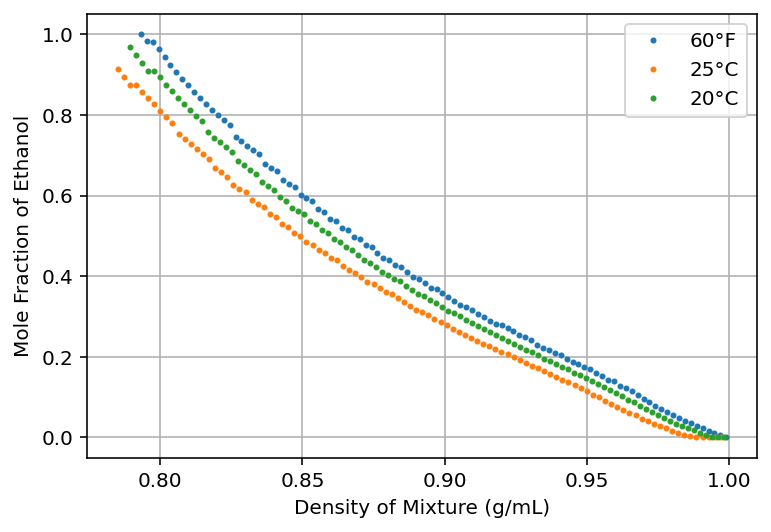
\includegraphics[width=1in,height=1.25in,clip,keepaspectratio]{fig1}}]{Michael Shell}
		Use $\backslash${\tt{begin\{IEEEbiography\}}} and then for the 1st argument use $\backslash${\tt{includegraphics}} to declare and link the author photo.
		Use the author name as the 3rd argument followed by the biography text.
	\end{IEEEbiography}
	
	\vspace{11pt}
	
	\bf{If you will not include a photo:}\vspace{-33pt}
	\begin{IEEEbiographynophoto}{John Doe}
		Use $\backslash${\tt{begin\{IEEEbiographynophoto\}}} and the author name as the argument followed by the biography text.
	\end{IEEEbiographynophoto}
	
	
	
	
	\vfill
	
\end{document}


